\documentclass{standalone}
\usepackage{tikz}
\usepackage{ctex,siunitx}
\usepackage{tkz-euclide}
\usepackage{amsmath}
\usetikzlibrary{patterns, calc}
\usetikzlibrary {decorations.pathmorphing, decorations.pathreplacing, decorations.shapes,}
\begin{document}
\small
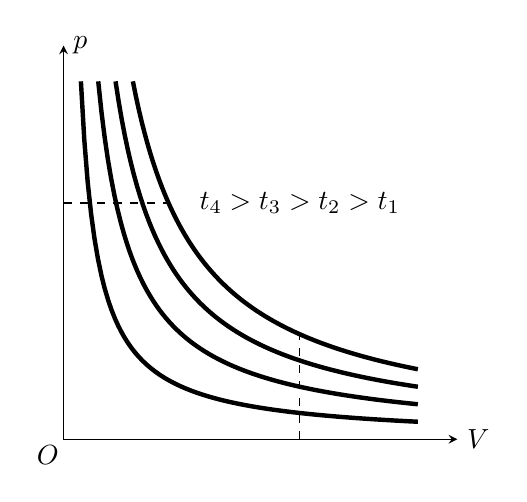
\begin{tikzpicture}[>=stealth, samples=100]
  \draw[<->] (0,5)node [right]{$p$}--(0,0)--(5,0) node [right]{$V$};
  \draw[color=black, ultra thick] plot[domain=0.22:4.5] (\x,{1/\x}) ;
  \draw[color=black, ultra thick] plot[domain=0.44:4.5] (\x,{2/\x}) ;
  \draw[color=black, ultra thick] plot[domain=0.66:4.5] (\x,{3/\x}) ;
  \draw[color=black, ultra thick] plot[domain=0.88:4.5] (\x,{4/\x}) ;
  \draw [dashed] (0,3)--(4/3,3);
  \draw [dashed] (3,0)--(3,4/3);
  \node at (-.2,-.2){$O$};
  \node at (3,3){$t_4>t_3>t_2>t_1$};
\end{tikzpicture}
\end{document}